\documentclass[a4paper]{article} %style de document
\usepackage[utf8]{inputenc} %encodage des caractères
\usepackage[french]{babel} %paquet de langue français
\usepackage[T1]{fontenc} %encodage de la police
\usepackage[top=2cm,bottom=2cm,left=2cm,right=2cm]{geometry} %marges
\usepackage{graphicx} %affichage des images
\usepackage{hyperref}%rend actif liens et références
\usepackage{verbatim}%permet insertion de texte brut (du style le logo Latex)
%\usepackage{amssymb} %collection de symboles
\usepackage[dvipsnames]{xcolor}%importe les couleurs, l'option permet d'avoir encore plus de couleurs
\usepackage{sectsty}%permet de changer les couleurs des sections/titres, etc
\usepackage{tikz}%pour faire des figures
\definecolor{astral}{RGB}{46,116,181}
\sectionfont{\color{red}}
\subsectionfont{\color{Blue}}
\subsubsectionfont{\color{NavyBlue}}
\usepackage{appendix} % Pour l'annexe


\title{
\LARGE{\em{Rapport Conception de Logiciels}}\\\vspace*{0.5cm}
UE Conception de Logiciels\\
Licence Informatique
}
\author{
Elie M - A.L - E.G\\
\small{{ }}\\\vspace*{1cm}
Groupe 1B\\
Sujet : Optimisateur de Wargame
}

\date{2018 - 2019}

\begin{document} %début du document
\maketitle{\begin{center}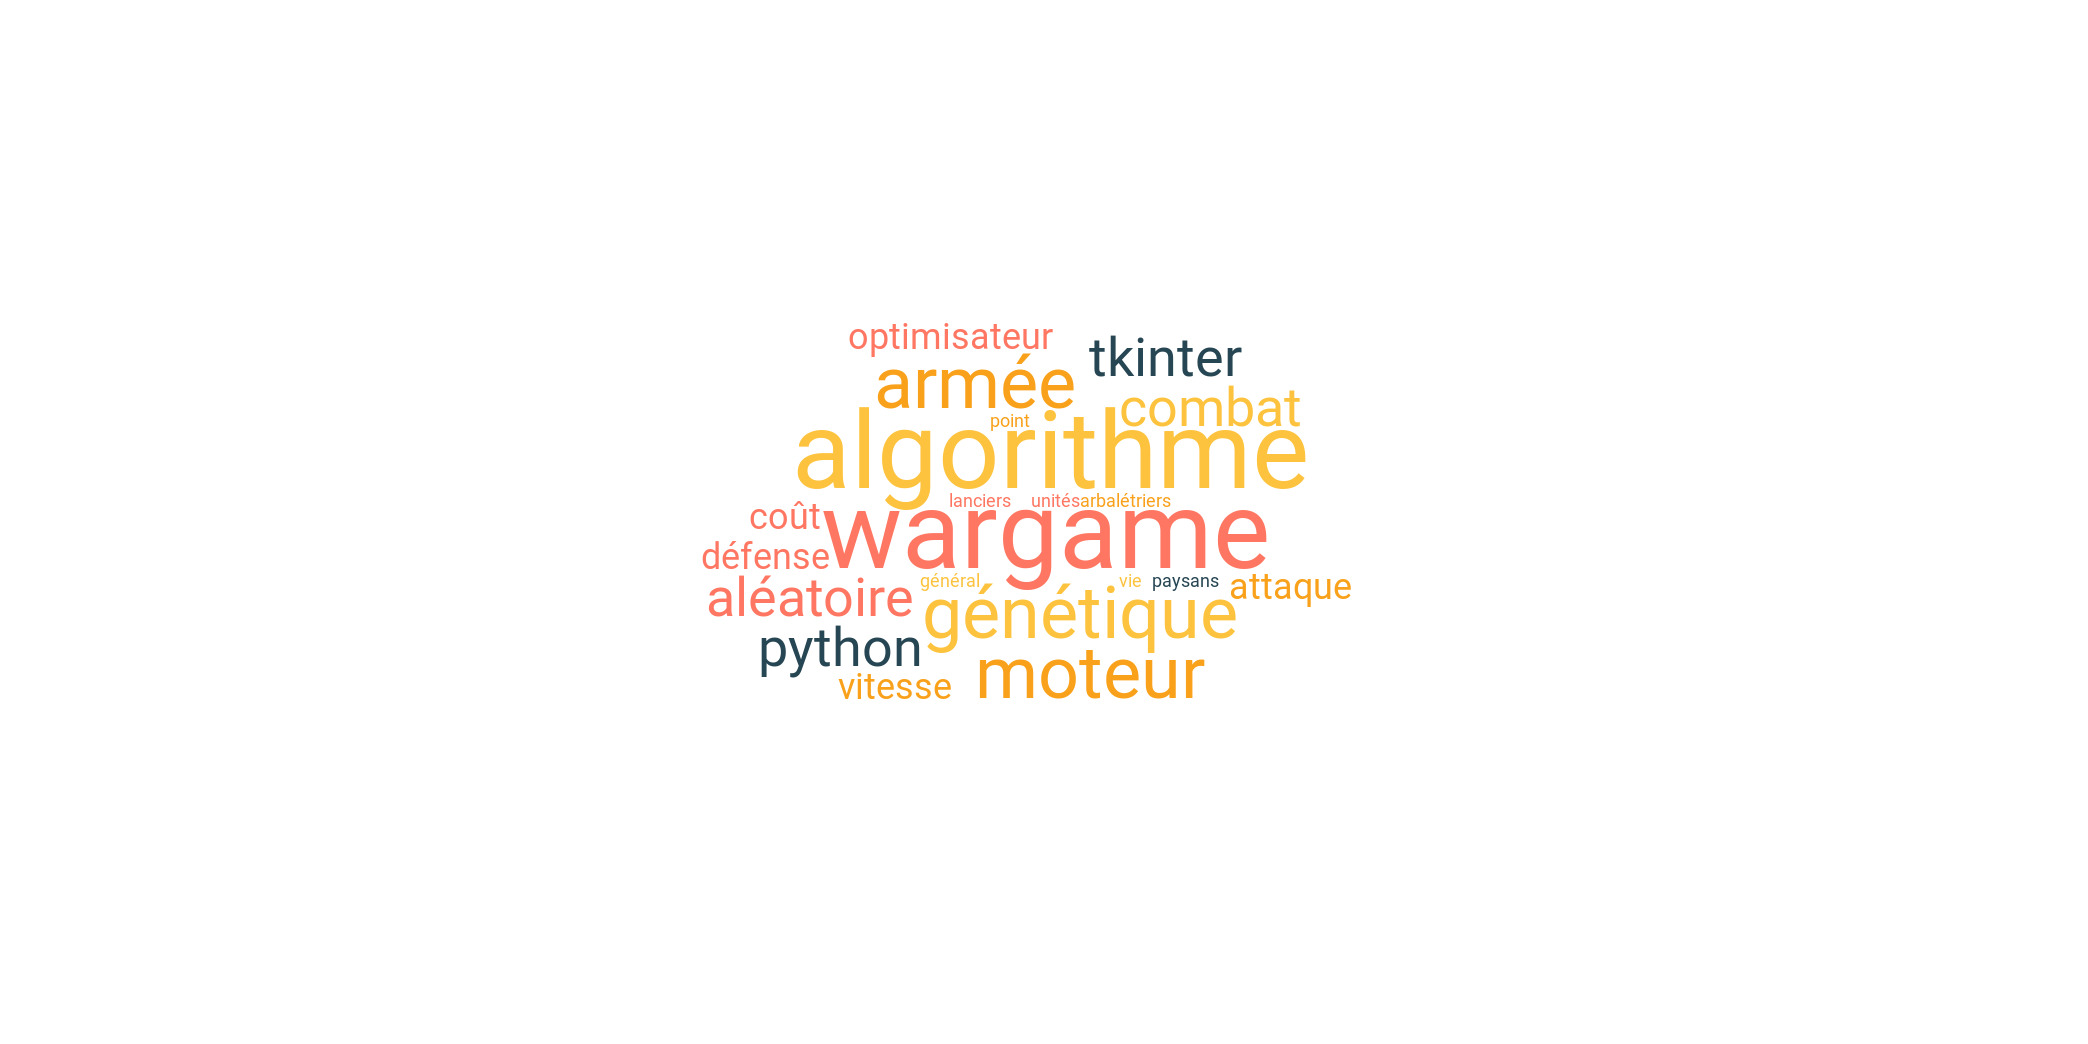
\includegraphics[width=18cm]{Images/Rapport_front_page.jpg}\end{center}}
\newpage
\newpage
	\null % Page blanche après page de garde
\newpage

\tableofcontents
\newpage

\section{Introduction}
\textit{"Shall we play a game"}, Joshua dans le film Wargames de 1983.
\medbreak
Quand nous avons vu le sujet du wargame en début d'année, nous avons tout de suite pensé à cette phrase mythique prononcée par le superordinateur de l'armée américaine dans le légendaire film des années 80 : Wargames. 
\smallbreak
C'est donc avec plaisir que nous avons décider de travailler dessus.
\smallbreak
Mais au fond qu'est-ce qu'un wargame ? Un wargame est à la base un jeu de plateau se jouant avec des figurines. C'est un jeu de guerre simulant des conflits entre plusieurs armées. Depuis le VIIe siècle, il est utilisé par les militaires comme outil de simulation et d'aide à la décision. De nos jours, c'est aussi un jeu de stratégie informatique. Le but est de détruire l'armée adverse en utilisant stratégie et tactique.

\section{Objectifs du projet}	
	\subsection{Ce qu’il fallait faire}
Le projet a été réalisé par A.L , E.G  et Elie M. Nous avons décidé en commun de créer un optimisateur de Wargame.
\\
Notre choix s'est naturellement porté vers ce sujet en raison de l'intérêt porté à sa thématique ainsi qu'à la mise en place d'un algorithme génétique.
Les objectifs du projet étaient multiples :
\begin{itemize}
        \item Créer un moteur de combat entre plusieurs armées avec des règles simplifiées
        \item Avoir un générateur automatique d'armées respectant une limite de points
        \item Développer un optimisateur d'armées issu d'un algorithme génétique
\end{itemize}
Comme le thème du wargame est ancien, on retrouve un certain nombre de jeux autour de cet univers. Regardons rapidement quelques exemples.

	\subsection{Ce qui existe déjà}
Des jeux de plateau dont Warhammer et Warhammer 40000 qui ont grandement popularisé le thème du wargame.
Mais aussi de nombreux jeux vidéos tirés de ce thème : Panzer General (1994), Warlords(1989), la série des Cossacks et des Age Of Empires, les jeux Paradox ou bien les jeux Total War.

Tous ont différentes manières d'aborder le wargame, avec ou sans plateau, représentation des combats en 2D et 3D, possibilité de placer ses troupes. Cependant, tous donnent la possibilité de créer son armée et de la faire affronter d'autres joueurs. Nous nous sommes donc centré sur ces points communs pour la base de notre jeu.

\section{Fonctionnalités implémentées}
Au cours du projet, de multiples fonctionnalités ont été implémentées. Il est possible de jouer seul via le Menu Solo de l'interface où l'utilisateur peut choisir son armée et de combattre une armée aléatoire ou une armée générée depuis l'optimisateur. De plus, l'utilisateur peut récupérer l'armée construite par l'algorithme génétique via le Menu Optimisateur -\ref{InterfaceOptimisateur}- ou une armée enregistrée localement -\ref{enregistrerRecuperer}-.\\

Il est également possible de jouer en duo, chacun choisissant son armée pour se défier. Tous les joueurs peuvent, s'ils le souhaitent, générer une armée aléatoire -\ref{aléatoire}- par rapport à un nombre de points donné tout en suivant les limites imposées par le Wargame -\ref{limitesWargame}-.\\

D'autres fonctionnalités sont également possibles, comme l'enregistrement d'une armée dans un fichier, -\ref{enregistrerRecuperer}- différents affichages pour donner des informations sur les combattants -\ref{afficherCarac}- ou sur le fonctionnement du jeu -\ref{ReglesFaq}-. Pour finir, un bouton reset permet de réinitialiser les armées de tous les joueurs. Ces fonctionnalités sont détaillées dans les parties suivantes. Notons pour la suite du rapport que les unités sont les différents Combattants et les troupes le nombre d'unités.

	\subsection{Description des fonctionnalités}
Au sein de l'interface graphique, on retrouve un menu présentant les différents modes de jeu et fonctionnalités :
\begin{figure}[!h]
	\begin{center}
	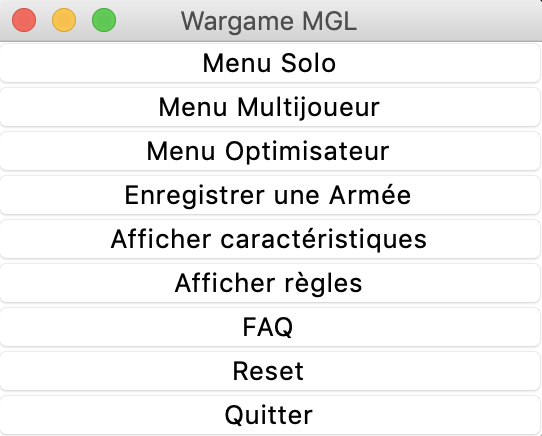
\includegraphics[width=6cm]{Images/interface.png}
	\caption{Menu principal\label{fig:MenuPrincipal}}
	\end{center}
\end{figure}

		\subsubsection{Menu Solo}
Le menu Solo permet de jouer contre l'ordinateur.
Le joueur peut créer une armée de différentes façons : manuellement, aléatoirement ou bien en utilisant l'algorithme génétique. La création aléatoire est basée sur le nombre de points que rentre l'utilisateur.
\begin{figure}[!h]
	\begin{center}
	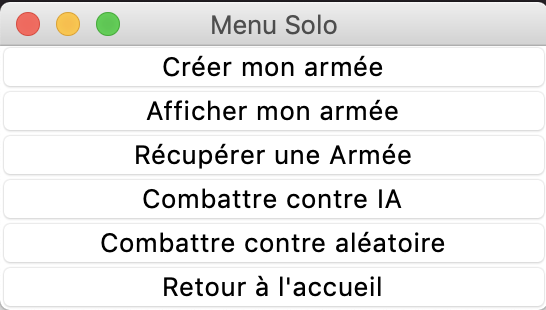
\includegraphics[width=6cm]{Images/menu1joueur.png}
	\caption{Menu solo\label{fig:MenuSolo}}
	\end{center}
\end{figure}

De plus, d'autres options s'offrent à l'utilisateur. Il peut afficher son armée et ses caractéristiques (même une armée vide), récupérer une armée enregistrée avec un nom ou depuis un explorateur de fichier. Cette dernière est enregistrée dans un fichier JSON qui comporte un effectif.\\

Enfin, quand l'utilisateur souhaite lancer le combat, deux possibilités s'offrent à lui : combattre contre une armée aléatoire ou contre une armée formée par l'IA.
Le vainqueur est ensuite déclaré par un écran de résultat.\\

Pour procéder à ces combats, l'interface stocke l'armée du joueur dans l'attribut de classe \texttt{armeeSolo} de la classe MaFen. Si l'utilisateur lance le combat contre l'aléatoire, une armée sera générée automatiquement avec le nombre de points de l'armée du joueur. Au contraire, si l'utilisateur choisi l'IA, l'armée doit être générée depuis l'optimisateur au préalable. Des tests permettent de ne pas déséquilibrer le nombre de points entre les deux armées. Ces deux armées sont ensuite envoyées dans le moteur de combat avant que le gagnant soit désigné. L'affichage correspondant apparaît après les écrans de bataille en cours. La méthode qui permet de lancer le combat est directement appelée lors du clic sur le bouton.

		\subsubsection{Menu Multijoueur}
Le menu Multijoueur permet de jouer avec un ami sur le même ordinateur.

\begin{figure}[!h]
	\begin{center}
	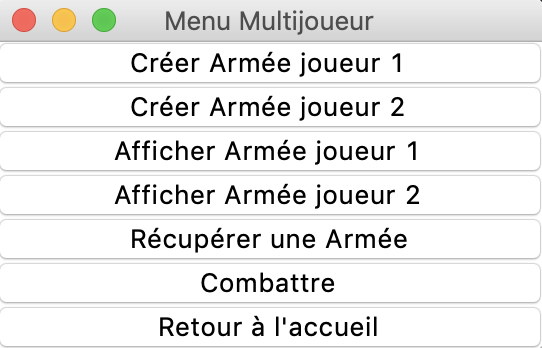
\includegraphics[width=6cm]{Images/menuMultijoueur.png}
	\caption{Menu multijoueur\label{fig:MenuMultijoueur}}
	\end{center}
\end{figure}

Il comporte la plupart des fonctionnalités du Menu Solo : création des armées de manière aléatoire ou grâce à l'algorithme génétique, affichage des armées, récupération d'une armée contenue dans un fichier JSON et lancement du combat entre les deux joueurs.

Les deux armées envoyées au moteur de combat sont situées dans les attributs de classe de MaFen : \texttt{armeej1} et \texttt{armeej2}. Le résultat est récupéré puis le vainqueur correspondant est affiché à l'écran.

Lorsque qu'une armée d'un des deux joueurs est créée, la seconde armée est bridée en nombre de points. Il est impossible de valider l'effectif tant que le nombre de points n'est pas inférieur ou égal au nombre de points de l'armée adverse. Cette limitation permet de ne pas déséquilibrer les combats.

		\subsubsection{Menu Optimisateur}
Le menu Optimisateur permet de créer une armée optimisée. En effet, cette armée disposera d'un nombre de combats victorieux conséquent. Une armée issue de cette optimisation a donc plus de chances d'obtenir la victoire. Cependant, cette probabilité de gagner dépend des paramètres choisis par l'utilisateur. Voici la page sur laquelle l'utilisateur choisit ces paramètres :

\begin{figure}[!h]
	\begin{center}
	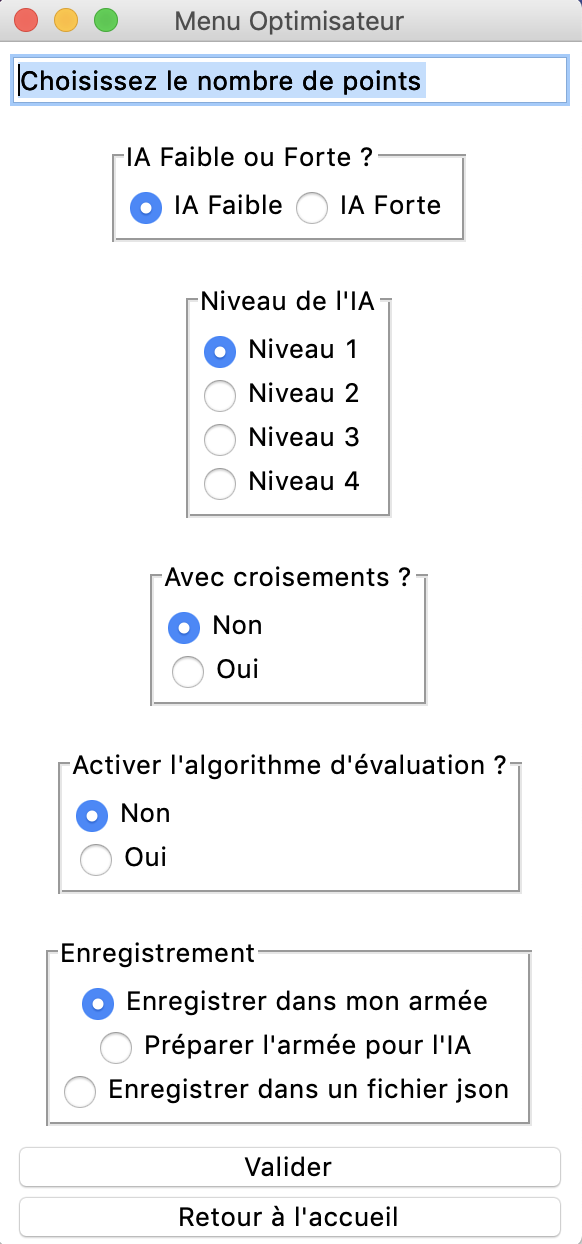
\includegraphics[width=5cm]{Images/menuOptimisateur.png}
	\caption{Menu optimisateur\label{fig:MenuOptimisateur}}
	\end{center}
\end{figure}

Tout d'abord, le joueur détermine le nombre de points des armées générées dans le champ d'entrée. 
Puis plusieurs options s'offrent à lui, modifiables à l'aide de boutons-radios des labelFrame.
\\
La première concerne la compétence de l'IA (faible ou forte) -\ref{OptiFaibleFort}-. Il faut également choisir entre quatre niveaux d'optimisation. Plus le niveau est haut, plus l'armée sera compétente et l'optimisation longue -\ref{OptiNiveaux}-.
\\
Ensuite, deux paramètres sont optionnels : l'ajout de croisements entre les armées -\ref{OptiCroisements}- et l'activation d'un algorithme d'évaluation -\ref{OptiEval}- qui se base sur le nombre de victoires d'une armée.\\

Si les croisements sont activés, le nombre de points de l'armée peut être légèrement modifié de $\pm 10\%$. Cette dérive n'a pas été gérée dans l'optimisateur car la forme des armées n'est pas adéquate à cette manipulation. Des tests ont été menés sans réel résultat.\\

L'algorithme d'évaluation indique à l'utilisateur si l'armée a réussi à passer un test de validité -\ref{OptiEval}-. Si ce n'est pas le cas, le joueur peut alors décider de recommencer ou non le processus.
\\
Enfin, l'utilisateur choisit où sauvegarder l'armée générée, pour le joueur solo, pour l'armée de l'IA ou directement dans un fichier JSON. La sérialisation se fait directement dans la méthode de lancement de l'algorithme. Mais il aurait été possible de créer une autre méthode pour effectuer cette tâche.\\

Les valeurs des boutons radios sont stockées dans des variables IntVar() et dans une variable StringVar() pour le nombre de points. Ces valeurs sont ensuite récupérées par la méthode de lancement de l'algorithme pour les passer au module optimisateur. De plus, une barre de chargement est lancée grâce à un deuxième Thread -\ref{InterfaceOptimisateur}-.

		\subsubsection{Enregistrer et récupérer une armée}\label{enregistrerRecuperer}
Le menu Enregistrer une armée permet de sauvegarder une armée dans un fichier JSON.\\

L'utilisateur donne un nom à son armée puis définit le nombre de troupes de chaque unité. Il est également possible de récupérer une armée courante d'un des joueurs et celle de l'IA. Cette récupération place la valeur des curseurs sur le nombre de troupes de chaque unité, il est possible par la suite de modifier ces valeurs.\\

La fonction la plus difficile à implémenter dans ce menu fut la création d'un fichier dans le bon répertoire avec l'effectif choisit par l'utilisateur. De plus, pour afficher les statistiques en cours de l'armée, cette dernière doit être créée à chaque changement de curseur pour ensuite récupérer les totaux et les afficher proprement dans les labels d'affichage. Pour finir, depuis le menu d'enregistrement d'armée, il n'est pas possible de créer des armées aléatoires car des problèmes d'affichage survenaient.

Ce menu d'enregistrement est identique au menu de création d'armée, l'option de récupération d'armée courante disparaît mais la génération d'armées aléatoires est possible.\\

\begin{figure}[!h]
	\begin{center}
	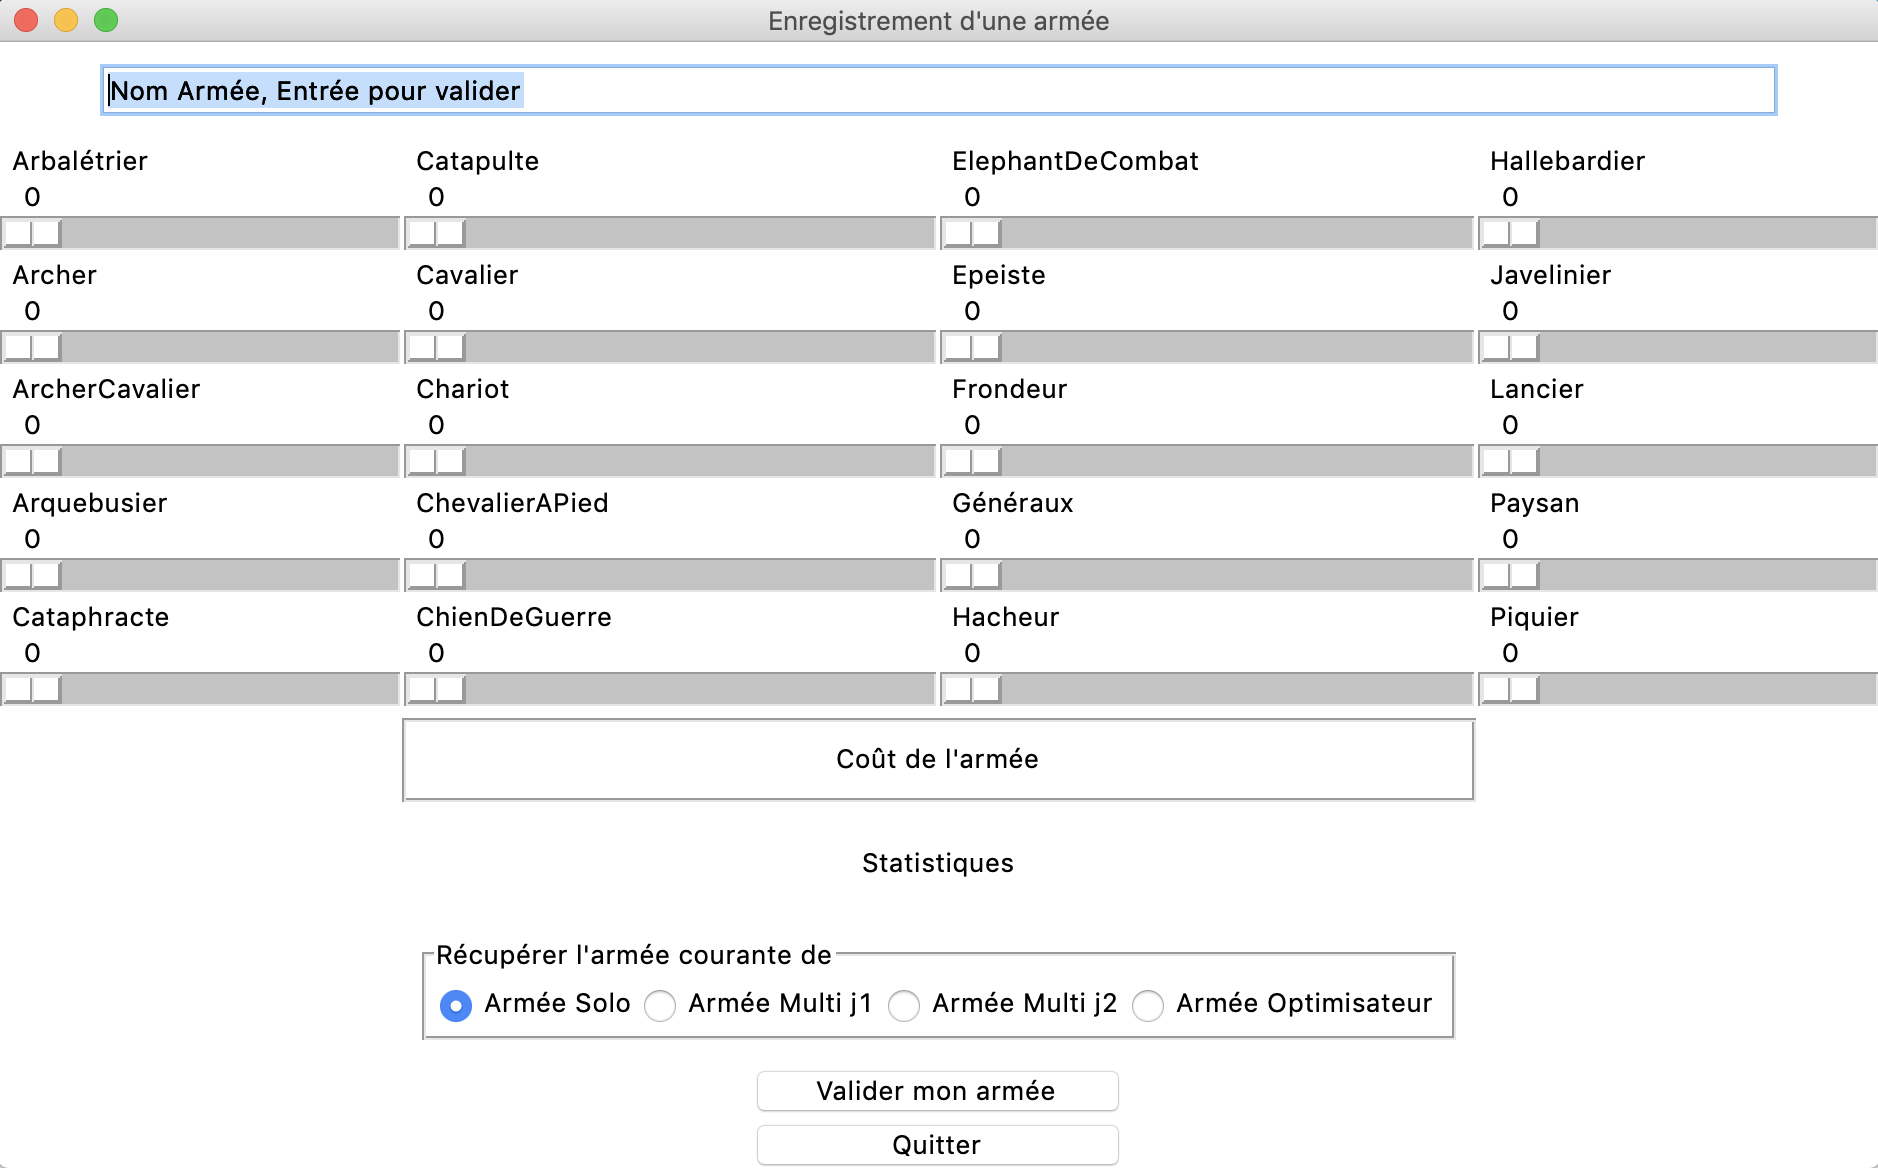
\includegraphics[width=11cm]{Images/enregistrerArmee.png}
	\caption{Enregistrement d'une armée\label{fig:EnregistrerArmee}}
	\end{center}
	\begin{center}
	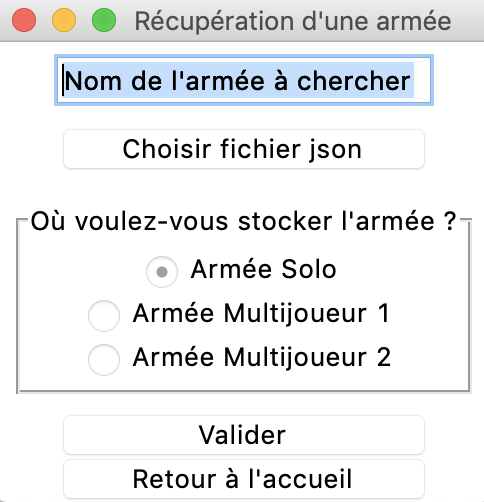
\includegraphics[width=4.5cm]{Images/recupArmee.png}
	\caption{Récupération d'une armée\label{fig:RecuperationArmee}}
	\end{center}
\end{figure}

La récupération d'armée fonctionne en concordance avec l'enregistrement. L'utilisateur donne un nom d'armée. Si elle est trouvée en tant que fichier JSON, alors elle est extraite, instanciée puis affichée pour validation par l'utilisateur. Si elle n'est pas trouvée, une pop-up apparaît pour signifier que l'armée n'existe pas car le chemin est incorrect. L'utilisateur peut aussi sélectionner directement le fichier via un explorateur, module de Tkinter qui renvoie le chemin de l'objet sélectionné. Lors de la récupération d'une armée, l'armée du joueur est modifiée, mais l'ancienne est stockée temporairement pour lui permettre de quitter sans enregistrer. Cette option était assez compliquée à mettre en place car le stockage de l'armée doit être fait en amont, puis il faut deux méthodes selon le choix de l'utilisateur pour valider ou non ce choix.

		\subsubsection{Afficher caractéristiques}\label{afficherCarac}
	Le menu Afficher caractéristiques permet d'afficher toutes les caractéristiques de toutes les unités. Les points de vie, de défense, d'attaque, de vitesse ainsi que leur coût sont indiqués en ligne par rapport au nom de la troupe.\\

L'index dans la hiérarchie de combat des unités est également affiché : cette hiérarchie indique l'ordre dans lequel les troupes succomberont lors d'un combat. D'autres informations supplémentaires sont affichées : les limites imposées lors de la création d'une armée et définie par la partie \ref{limitesWargame}.

L'affichage est réalisé dans une Toplevel de Tkinter. Elle est composée de séries de labels rangés dans une grille. Les informations sont issues de l'attribut de classe \texttt{carac} de la classe Troupe. Nous pouvons également noter que le chargement de cette Toplevel peut être long en raison du grand nombre de widgets. Toutes ces valeurs ont été décidées au début de notre projet, et dans un but d'équilibrer les unités entre elles.

\begin{figure}[!h]
	\begin{center}
	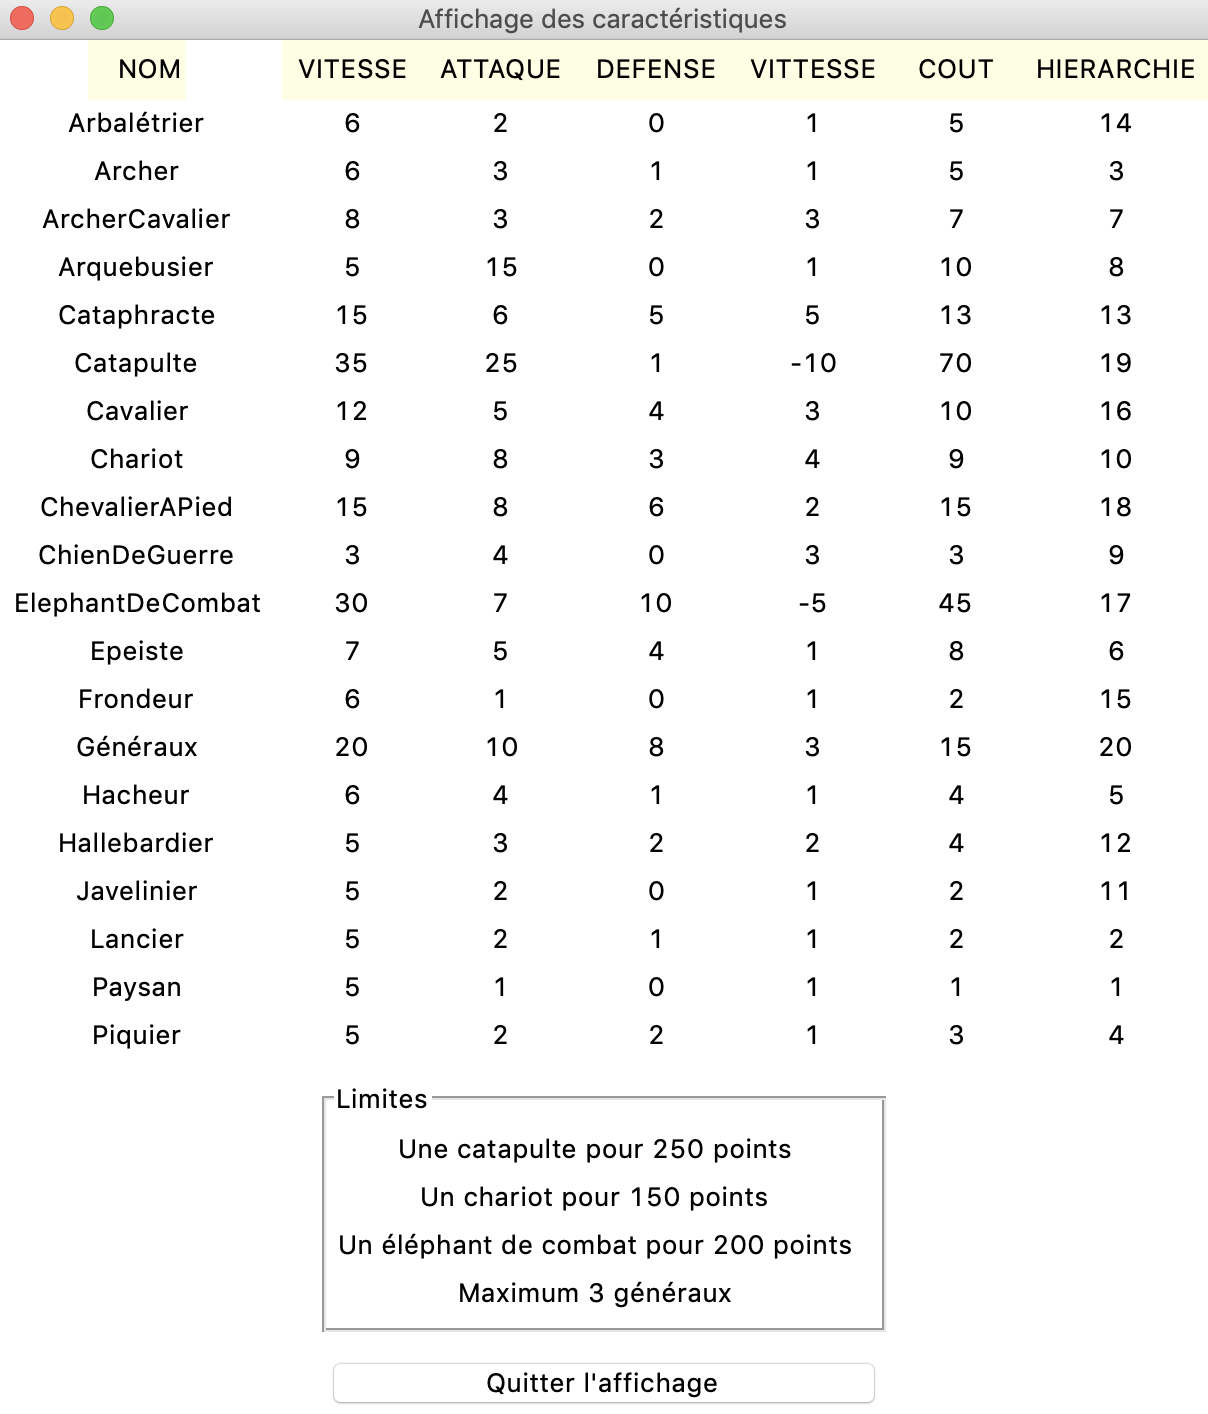
\includegraphics[scale= 0.4]{Images/afficherCaracteristiques.png}
	\caption{Affichage des caractéristiques des unités\label{fig:AfficherCaractéristiques}}
	\end{center}
\end{figure}

		\subsubsection{Règles et FAQ}\label{ReglesFaq}
Il est possible d'afficher les règles du jeu. 
\\
Celles-ci sont établies pour conditionner le fonctionnement du jeu et donner les possibilités de chaque joueur. Elle permettent également de comprendre le principe du Wargame. Ces règles doivent être respectées pour le bon déroulement du jeu.

Pour déterminer ces règles, nous avons décidé d'inclure les points importants sur le fonctionnement du jeu. Ces règles sont stockées dans un fichier texte et l'interface récupère son contenu pour l'afficher dans un label.

De même, la FAQ donne des indications aux joueurs sur la manière d'utiliser l'interface et l'optimisateur. Elle est également stockée dans un fichier texte. Un test permet de vérifier si les fichiers sont disponibles, sinon un message d'erreur apparaît.

		\subsubsection{Les limites imposées par le Wargame}\label{limitesWargame}

Certaines unités du jeu disposent de limites. Le choix des unités a été assez difficile et la façon de les prendre en compte, compliquée. En effet, nous avons décidé de fixer des limites à quatre unités : trois par rapport au nombre de points de l'armée et une limite fixée.\\

La limite fixée s'applique à l'unité "Généraux", avec un maximum de trois troupes dans l'armée du joueur.\\

Les unités "Catapultes", "Éléphants de combat" et "Chariots" sont limitées respectivement à une troupe pour 250, 200 et 150 points. Ces limites s'appuient donc sur le nombre de points de l'armée et doivent être calculées à chaque modification de l'effectif.
\\
L'interface calcule ces limites, puis change la valeur maximale des curseurs des unités concernées. Les limites fixées sont stockées dans le dictionnaire \texttt{limites} de l'armée.

\begin{figure}[!h]
\begin{center}
\begin{tabular}{|l|c|}
  \hline
  Nom unité & Limitations\\
  \hline
  Généraux & Maximum 3 \\
  Catapultes & 1 pour 250 points \\
  Éléphants de combat & 1 pour 200 points \\
  Chariots & 1 pour 150 points \\
  \hline
\end{tabular}
\end{center}
	\caption{Tableau des limites de troupes\label{tab:limitesTroupes}}
\end{figure}

Ces limites d'unités ont également dû être ajoutées à la génération d'armées aléatoires.

	\subsection{Fonctionnalités abandonnées}
Au cours du projet, nous avons été amenés à revoir nos choix de départ afin d'améliorer le code produit. Voici plusieurs exemples qui illustrent notre évolution : 
\begin{itemize}
	\item Nous avions débuté par la conception des troupes avec une classe par troupe, créant un objet spécifique pour chacune d'entre elles (un objet Archer, un objet Chevalier...). Ce système n'était pas pratique car l'ensemble des unités disposaient des mêmes propriétés à l’exception de ses compétences.
	\item Notre première fonction aléatoire n'était pas optimisée car elle calculait le nombre maximum d'unités d'une troupe prise au hasard dans les troupes possibles. Puis elle générait aléatoirement un nombre entre 0 et ce maximum pour déterminer le nombre d'unités à former. Il pouvait ainsi y avoir les trois quarts d'une armée composée d'une seule troupe. Cette génération aléatoire a été abandonnée. Description de la nouvelle méthode dans la figure \ref{fig:DiagrammeAleatoire}.
	\item Il est possible d'ajouter une unité en exécutant des fonctions qui demandent en ligne de commande à l'utilisateur ses caractéristiques. Cependant, cette option est compliquée à mettre en place dans l'interface. La méthode de lancement d'une armée avec un ajout d'unité est la méthode \texttt{armee\_console} de la classe \texttt{Armee}.
\end{itemize}

	\subsection{Organisation du projet}
L'organisation du projet s'est déroulée en plusieurs étapes importantes, la première concerne la structure du projet. Plusieurs séances ont été consacrées au choix des unités, de la méthode de combat et notamment de la forme des batailles. En effet, deux pistes étaient possibles. Soit les troupes seraient disposées sur un plateau de jeu selon le choix de l'utilisateur, soit le combat serait purement calculatoire. Nous avons opté pour la partie calculatoire sans le plateau de jeu. De plus, nous avons décidé que la partie graphique serait faite en Tkinter.\\

En seconde phase du projet, E a pris les devants en débutant la programmation. En effet, A et Élie n'avaient pas d'expérience en programmation orientée objet contrairement aux notions que possédait déjà E. Les premiers tests se sont révélés concluants mais la maintenabilité du code était à revoir.\\

Après quelques séances, A a effectué la factorisation du code qu'avait écrit E à l'aide de boucles ; l'utilisation de dictionnaires était plus judicieuse et les combattants ne seraient plus des objets issus de diverses classes mais d'une seule (Troupe). Un héritage de classe s'est mis en place mais fut finalement abandonné en fin de projet car non pertinent.\\

À partir de ce moment, le projet s'est scindé en deux parties : A et Élie travaillaient sur la création d'une armée aléatoire et sur l'implémentation du moteur de combat pendant que E travaillait sur la réalisation de l'algorithme génétique.\\

Une première version du projet était fonctionnelle en console et permettait de choisir son armée, d'ajouter des unités et de s'affronter. Cependant, des modules de fonctions permettaient de faire ces combats. On avait donc un mélange de programmation impérative et objet car les fonctions travaillaient sur les objets et n'appelaient pas de méthodes propres aux armées. Ce défaut a été corrigé par la suite\\

Après cela, deux parties graphiques ont été codées par Élie et A. L'envie de saisir le fonctionnement de Tkinter était primordial pour faire une interface graphique. Après concertation, nous avons décidé de garder et de travailler uniquement sur la partie graphique d'A. Cette dernière ajoute de nouvelles fonctionnalités aux utilisateurs et permet par exemple d'enregistrer des armées ou de lancer une optimisation d'armées. Cependant, nous avons abandonné l'ajout de boutons sur des images de Élie, car trop compliqué à mettre en place.\\

Vers début mars, l'algorithme génétique a été ajouté à l'interface graphique. De légères corrections ont été apportées par toute l'équipe pour être le plus performant possible.\\

En dernière phase, le module \texttt{creationArmee} qui permettait jusqu'ici de créer les armées a été supprimé par A en ajoutant ces méthodes aux Armées, une programmation alors plus orientée objet. Les troupes héritaient également d'un objet Combattant, mais ce dernier n'avait pas d'utilité car l'héritage était inutile.\\

Les dernières modifications du code partaient notamment sur les DocStrings des fonctions et la mise aux normes PEP8. A a également ajouté les photos des résultats et un écran de combat pour simuler sa durée.\\

En ce qui concerne l'écriture du rapport et la présentation beamer pour la soutenance, Élie en a rédigé une grande partie, soutenu par les interventions d'A et d'E.

\section{Éléments techniques}
Les éléments techniques concernent principalement trois domaines :
\begin{enumerate}
	\item \hyperref[Algorithmes]{Les différents algorithmes}
	\item \hyperref[structureDonnees]{Les structures de données}
	\item \hyperref[bibliothèques]{Les bibliothèques utilisées}
\end{enumerate}

Dans l'ordre, voyons en détail chacun d'entre eux.

	\subsection{Algorithmes}\label{Algorithmes}
Les algorithmes sont au centre du programme. En première partie nous verrons l'algorithme issu du moteur de combat, puis deux méthodes de création aléatoire d'armées et de enfin l'algorithme génétique de l'optimisateur. Pour finir, nous présenterons le fonctionnement  de l'interface graphique.

		\subsubsection{Algorithme du moteur de combat}\label{moteurCombat}
Le moteur de combat permet de gérer l'affrontement de deux armées. Il détermine un vainqueur après avoir fait combattre les armées avec des règles simplifiées. Il est également possible d'obtenir une égalité.
\\
Le moteur de combat fonctionne uniquement avec deux armées passées en paramètre de la fonction moteur\_de\_combat du module \texttt{moteurCombat}. Ces deux paramètres sont appelés \texttt{armée\_1} et  \texttt{armée\_2}. Celles-ci doivent être des copies d'armées dans le but d'éviter de modifier les armées originales. En effet, le moteur de combat renvoie une valeur correspondante à l'index de l'armée passé en paramètre mais supprime les troupes dans les armées durant le combat.

Ces copies doivent être réalisées avant d'appeler la fonction, mais on aurait pu ajouter cette copie directement dans le moteur de combat.

Si l'on travaille sur l'armée originale, le programme élimine les troupes et l'armée gagnante ne pourrait plus être utilisée car elle serait incomplète.

De plus, le moteur de combat fonctionne au tour par tour. \\

Premièrement, nous construisons une hiérarchie qui va nous permettre de retirer dans un certain ordre les unités de l'armée. Puis nous effectuons une comparaison de la vitesse totale de l'armée 1 et de l'armée 2. Celle qui a l'avantage gagne un bonus d'attaque de $2.5\%$. Si les deux armées ont la même vitesse, une armée est choisie aléatoirement pour bénéficier du bonus d'attaque. Le schéma explicatif : Figure \ref{fig:DiagrammeMoteurCombat}

Tant qu'une armée n'est pas vaincue nous continuons le combat. Une boucle while not teste à chaque itération si une armée est battue, c'est à dire qu'elle ne dispose plus de troupes. A partir de là nous regardons le total de dégâts infligés par les deux armées. Celui-ci est calculé par le total de point d'attaque de l'armée adverse moins le total de sa défense. Ainsi, il faut toujours que le nombre de points d'attaque d'une unité soit supérieure à sa défense.

A partir de là, nous retirons les morts de chacune des deux armées. Après avoir retiré les unités des armées, il est possible qu'un reste d'attaque existe. Celui-ci est sauvegardé temporairement et ajouté au total de l'armée lors du prochain tour. Cela permet d'éviter d'avoir des combats où des unités n'arrivent pas à se tuer mutuellement car elles ont trop de points de vie et de défense.\\

Le calcul des totaux est effectué et la variable tour s'incrémente.
Si un combat dure trop longtemps, alors nous arrêtons le programme et nous disons que c'est une égalité.\\

Voici un diagramme qui illustre son fonctionnement global. Figure :  \ref{fig:DiagrammeMoteurCombat}
\begin{figure}[!h]
	\begin{center}
	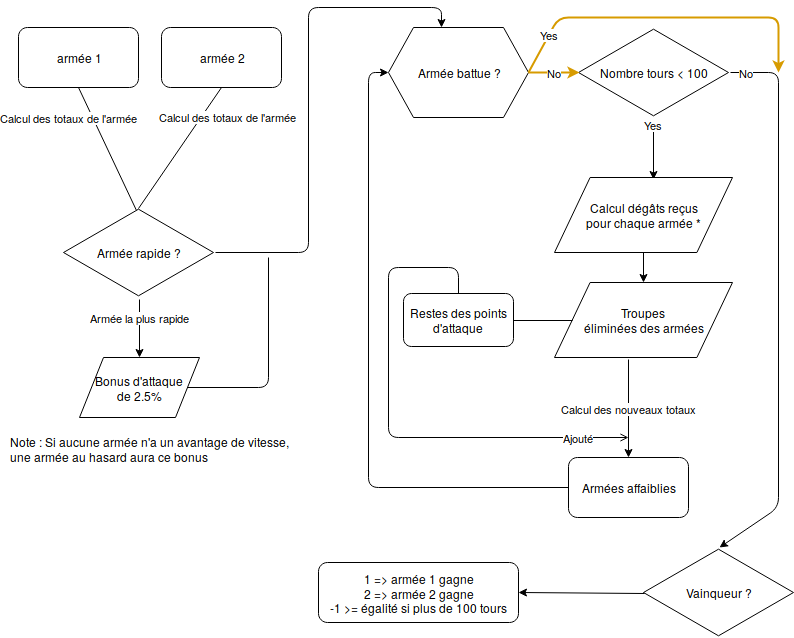
\includegraphics[width=12cm]{Images/Diagramme_moteur_combat.png}
	\caption{Fonctionnement du moteur de combat\label{fig:DiagrammeMoteurCombat}}
	\end{center}
\end{figure}

		\subsubsection{Algorithme de la création aléatoire d'armées}\label{aléatoire}
La possibilité de gérer des armées a été au cœur de notre discussion au début du projet. En effet, il nous fallait trouver une ou plusieurs méthodes qui permettai(en)t d'avoir des armées variées. Ces armées allaient ensuite être utilisées dans le cadre de l'algorithme génétique.\\

Deux fonctions issues de \texttt{Armee.py} nous permettent de créer des armées aléatoires. La première a été abandonnée. Le problème majeur sur cette dernière était qu'il y avait peu de diversité au sein de l'armée. De plus, le nombre de points totaux n'était souvent pas atteint. Cela était dû au fait que la fonction choisissait un nombre au hasard entre le minimum et le maximum d'une unité qu'il était possible de recruter. Une armée pouvait donc être composée au trois quart d'une seule unité.\\

La deuxième méthode est bien plus intéressante à ce niveau. Ici, nous prenons une unité au hasard et nous ajoutons à l'armée une seule troupe de cette unité - si possible en fonction des limites imposées. Si une troupe dispose d'une limite, comme les généraux (trois au maximum), cela est pris en compte et il n'est pas possible d'en avoir plus. L'armée se construit donc plus lentement mais peut disposer d'une large variété d'unités ainsi qu'un nombre de points toujours égal au nombre de points demandé. La fonction renvoie un dictionnaire, préalablement vide, contenant tous les types d'unités (clé) ainsi que leur nombre (valeur).\\

Voici une Figure : \ref{fig:DiagrammeAleatoire} qui illustre les deux types de formation d'armées. Notons que seule la deuxième méthode est conservée car elle est plus efficace.
\begin{figure}[!h]
	\begin{center}
	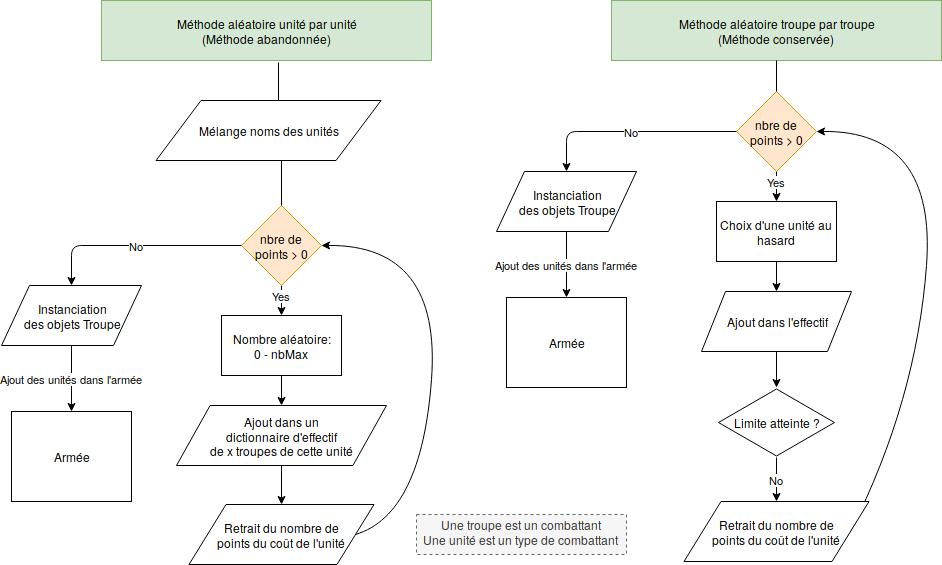
\includegraphics[width=14cm]{Images/creation-armee.png} 
	\caption{Fonctionnement du moteur de combat\label{fig:DiagrammeAleatoire}}
	\end{center}
\end{figure}

		\subsubsection{Algorithme génétique}\label{AlgoGen}
Le schéma ci-dessous vous présente le fonctionnement général d'un algorithme génétique au sein duquel on retrouve un certain nombre de possibilités dans le choix des fonctions.

\begin{figure}[!h]
	\begin{center}
	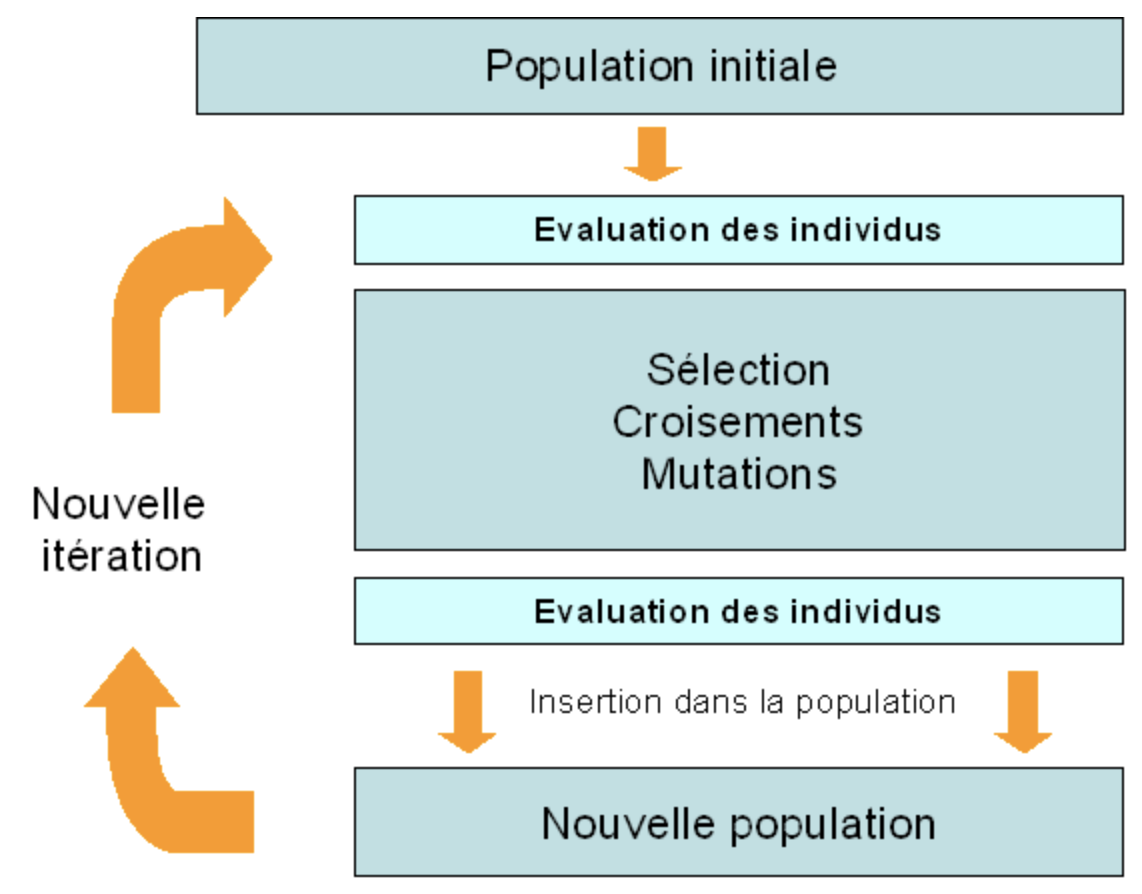
\includegraphics[scale= 0.4]{Images/algoGenet.png}
	\caption{source : \href{https://khayyam.developpez.com/articles/algo/genetic/\#L3.3}{developper.com}}
	\end{center}
\end{figure}

Bien entendu, ce schéma peut, et souvent doit, être modifié en fonction du contexte, ce qui est le cas ici. En effet, on ne cherche pas à obtenir une population d'armées performantes mais une seule et unique armée.\\

C'est ainsi que nous avons décidé d'utiliser la sélection par tournois, le croisement multi-points ainsi qu'un algorithme d'évaluation. On aurait pu ajouter d'autres méthodes de sélection comme la roulette, la sélection par rang ou encore la mutation génétique post-sélection. Elles pourraient compléter l'algorithme dans une autre version du jeu où le temps d'exécution, déjà bien long dans certains cas, aurait été encore plus maximisé.\\

\label{OptiFaibleFort}On débute donc le processus avec la création d'une population initiale (une population composée d'armées). Deux choix sont possibles pour l'utilisateur : une population de départ normale ou une population de départ évoluée (c'est-à-dire que chaque armée la composant a déjà passé un certain nombre de tests et est donc considérée comme semi-performante). Ce choix correspond à la partie "IA Faible ou Forte" de l'interface graphique.\\

On enchaîne ensuite avec la Sélection par Tournois, conçue de la même manière que nous le ferions dans la réalité : des championnats départementaux, des championnats régionaux qui verront s'affronter les meilleures de chaque département, des championnats nationaux qui verront s'affronter les meilleures de chaque région et enfin les championnats mondiaux qui verront s'affronter les meilleures de chaque nation. Ce sont-là de simples repères dans l'organisation de l'algorithme.
Le champion départemental sera sorti vainqueur d'un tournoi opposant seize armées d'une population initiale. Le championnat régional sera le terrain d'affrontement de seize armées multiplié par le nombre de départements voulus par le joueur et ainsi de suite jusqu'au championnat mondial (16 départementaux x 16 régionaux x 16 nationaux +1).\\

\begin{figure}[!h]
	\begin{center}
	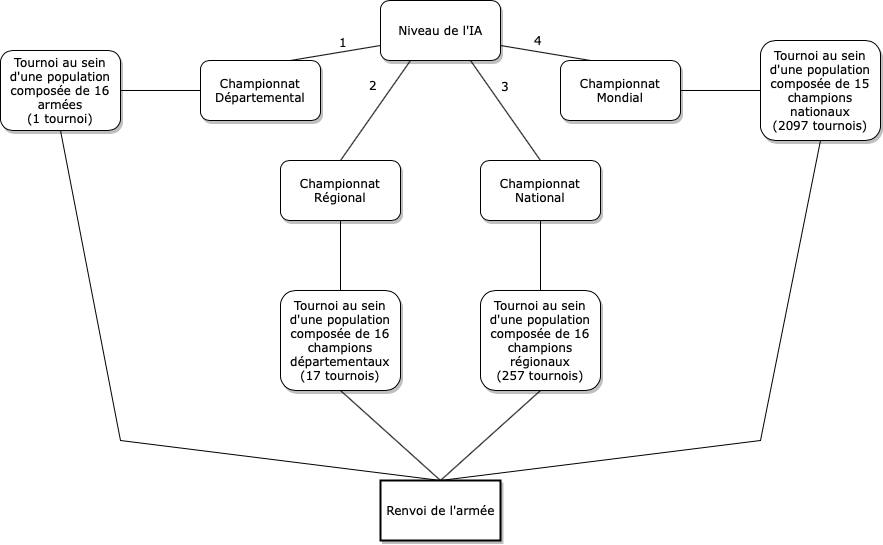
\includegraphics[scale= 0.5]{Images/Championnats.png}
	\caption{Schéma représentant la partie Sélection par Tournois}
	\end{center}
\end{figure}

On choisit le nombre 16, non paramétrable par le joueur, bien que cela pourrait être un ajout supplémentaire. En effet, il s'agit du nombre le plus simple à utiliser pour l'algorithme de gestion des tournois (étant un multiple de 2 supérieur à 8) et également pour la vitesse d'exécution déjà très lente dans le cas où l'utilisateur choisirait tous les paramètres optimaux pour l'IA.\\

\label{OptiNiveaux}Ainsi, quatre niveaux sont mis à la disposition du joueur pour l'optimisateur. Le niveau 1 correspond à un champion départemental. Le niveau 2, un champion régional. Le niveau 3, un champion national et enfin le niveau 4, un champion mondial.
A cet instant, on sait donc quel niveau nous devons utiliser et si les populations de départ doivent être évoluées ou non.\\

\label{OptiCroisements}Vient après cela la fonction gérant le croisement multi-points. On commence par créer deux armées selon les paramètres fixés par le joueur (Faible ou Forte, Niveau). Nous prenons ensuite les deux premières parties des armées, les 10 premières troupes, puis on les interchange afin d'obtenir deux nouvelles armées ayant été croisées. On retourne la meilleure des deux, récupérée après un combat. Néanmoins, il fallait également prendre en compte le fait qu'un croisement de ce type risquait de modifier les points totaux des armées et de s'éloigner de la demande de l'utilisateur. C'est la raison pour laquelle nous avons fixé un plafond de 10\% à respecter. Si ce n'est pas le cas, l'algorithme recommencera alors le même schéma depuis la création des deux armées.

\label{OptiEval}Par la suite, on s'intéresse aux performances de l'armée obtenue. Pour cela, un algorithme d'évaluation a été conçu. Ainsi, il va soumettre l'armée optimisée à une série de combats contre d'autres armées. Si elle parvient à remporter un tiers d'entre eux, alors elle est considérée comme performante. Le nombre de combat qu'elle aura à mener va dépendre du niveau de l'IA choisi par le joueur. Au niveau 1, elle devra livrer 10 combats. Le niveau 2, 20 combats... etc.\\

Ainsi, notre algorithme génétique possède les fonctionnalités suivantes : création de populations initiales évoluées ou non (Faible ou Forte), sélection par tournois (en fonction du niveau), croisement multi-points, algorithme d'évaluation, tous pouvant être choisis ou non par le joueur ce qui offre un bon niveau de paramétrabilité pour l'optimisateur.

\begin{figure}[!h]
	\begin{center}
	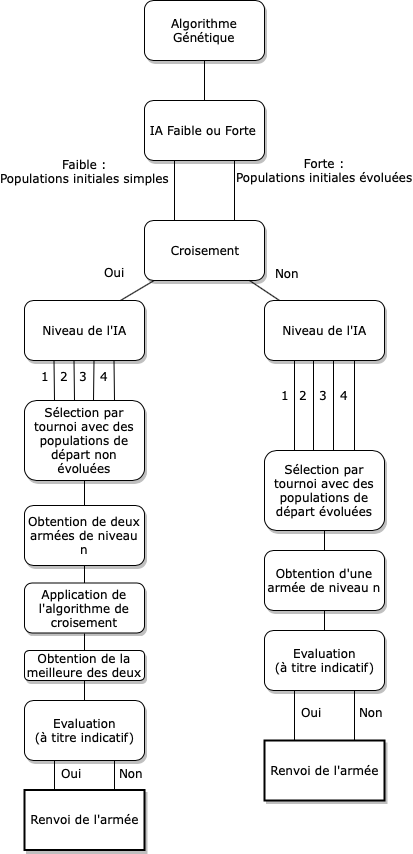
\includegraphics[scale= 0.5]{Images/AlgorithmeGenetique.png}
	\caption{Schéma représentant l'ensemble de notre algorithme génétique}
	\end{center}
\end{figure}

L'ensemble de l'algorithme génétique a été conçu à la main dans un souci d'apprentissage, sans utilisation de bibliothèques spécialisées. Cela pourrait être une amélioration pour raccourcir le temps d'exécution de l'optimisateur.

		\subsubsection{Algorithme de la partie graphique}\label{algoInterface}
La partie graphique est le fichier le plus volumineux. En effet, il dépasse les milles lignes de code.\\

La partie graphique utilise la programmation objet. Ainsi, dix-sept classes ont été déclarées dans le fichier \texttt{interface.py}. Les principales classes sont la fenêtre principale et celles qui permettent d'afficher les différents menus (Solo, Multijoueur, Optimisateur, Règles, FAQ, etc). D'autres classes comme EnregistrerArmee servent à la fenêtre principale pour les différentes fonctions proposées.\\

La fenêtre principale est la classe MaFen, elle hérite de l'objet Tk, qui est une fenêtre graphique Tkinter.
\\
Elle permet de gérer les actions de l'utilisateur en manipulant les classes. Elle comporte plusieurs attributs de classe, un dictionnaire troupes qui sert à stocker les effectifs temporaires des armées. Elle comporte également quatre objets Armee qui correspondent aux armées des joueurs solo, duo(joueur 1 et joueur 2) et celle de l'optimisateur. Ces attributs sont accessibles facilement via \texttt{MaFen.armeeSolo}.\\

Ensuite, cette classe comporte des attributs d'instance, dont notamment un dictionnaire \texttt{frames} qui contient les différentes frames possibles pour l'affichage. Ce sont des objets issus des classes correspondantes aux menus et frames de résultat ou à la  création/récupération d'armée. Ces objets ont hérité de la classe Frame. Ce système permet d'afficher dans la fenêtre principale les frames selon le choix de l'utilisateur. Ainsi, au lancement de l'application se crée l'ensemble des frames. Elles sont stockées dans le dictionnaire pour rapidement les utiliser par la suite. 
Au démarrage, la page d'accueil est affichée. C'est ce que l'utilisateur verra quand il ouvrira le programme. \\

Dans cette page d'accueil, plusieurs boutons permettent d'aller dans les différents sous-menus.
\\
Pour changer de frame, la méthode \texttt{changer\_frame} de la classe \texttt{MaFen} va oublier la frame actuelle contenue dans l'attribut \texttt{currentFrame} et ajouter la nouvelle via la méthode \texttt{pack()}. Pour finir, la nouvelle frame est placée en référence dans l'attribut \texttt{currentFrame}.\\

Chaque menu peut contenir des widgets : des boutons, boutons-radio, labels ou encore des canvas pour afficher les images. Chacun de ces widgets, objets de Tkinter, doit être instancié puis ajouté via la méthode \texttt{pack()} ou \texttt{grid()} selon l'arrangement de la frame. Ils sont donc visibles sur la frame quand elle est ajoutée à la fenêtre principale. Par exemple, pour ajouter un bouton dans une frame, on écrira : \texttt{Button(self, ses options).pack()}.\\

À ce titre, le bouton Reset de la page d'accueil est particulier. En effet, celui-ci ne renvoie pas vers une autre page mais réinitialise les armées (on instancie de nouveaux objets Armee pour tous les joueurs). En appuyant sur le bouton, celui-ci exécute la méthode de classe \texttt{reset}. Les armées des joueurs Solo, Multijoueur et Optimisateur sont remises à zéro. Cette méthode est déclarée comme \texttt{@classmethod} car elle n'effectue pas de changement sur l'objet mais sur les attributs de classe.\\

Des événements claviers sont ajoutés, comme la touche "échap" pour quitter le jeu ou encore la touche "Entrée" pour valider rapidement dans les menus. Cependant, comme cette attribution de touche renvoie un paramètre supplémentaire lors de son appel, il faut ajouter \texttt{*args} dans les paramètres des méthodes concernées, puis utiliser ce paramètre avec la méthode statique \texttt{unused} pour éviter les erreurs de norme.\\

Les boutons Règles et FAQ renvoient vers une page (une frame) qui ouvre un fichier grâce aux fonctions \texttt{open} et \texttt{read}. Si le fichier est introuvable, il est indiqué à l'utilisateur que le fichier n'a pas été trouvé. Le test pour trouver le fichier est réalisé avec \texttt{os.path.isfile(link)} qui teste si le chemin existe dans l'ordinateur.\\

Avant de passer à l'algorithmie des pages issues du menu solo, multijoueur et optimisateur, voyons un autre bouton important : Enregistrer une armée. Grâce à ce bouton, l'utilisateur va pouvoir créer une infinité d'armées et les enregistrer.
Il va ensuite avoir la possibilité de les utiliser sur le champ de bataille via l'option de récupération d'armée.

La sélection d'une armée est commune aux frames EnregistrerArmee et NouvelleArmee, elle fait appel à la Frame SelectionTroupe en lui passant des paramètres supplémentaires.
En effet, selon les paramètres passées à l'instanciation, de nouveaux boutons apparaissent pour la sélection. 

Par exemple pour la création d'une nouvelle armée, on ajoute la Frame SelectionTroupes avec le paramètre alea : \texttt{SelectionTroupes(self, armee, alea=True)}. Un test dans la Frame SelectionTroupes permet d'ajouter le bouton de création aléatoire quand ce paramètre est passé. Pour récupérer ces mots clés supplémentaires, on test si ce mot est présent dans le dictionnaire $**kwargs$.

À l'inverse, pour l'enregistrement d'une armée, l'option de récupération est passée à la place de l'aléatoire : \texttt{SelectionTroupes(self, armee, recup=True)}. Cette option affiche un menu pour récupérer l'armée courante d'un des joueurs.\\

Une fois ce menu affiché, l'utilisateur choisit ses troupes, il fait glisser un curseur (Scale) pour choisir le nombre d'unités qu'il souhaite. Il existe cependant une limite de deux cents unités par troupe (ex: 200 cavaliers au maximum).
\\
A chaque changement de valeur d'un curseur, le nombre de troupes de l'unité est mis à jour dans le dictionnaire troupes de la classe MaFen. Une armée est instanciée puis les troupes sont ajoutées par rapport à cet effectif. Certaines informations comme ses statistiques apparaissent dans des Labels. On voit également si une limite est en cours pour le joueur adverse, pour ne pas déséquilibrer les armées. Des curseurs se trouvent bloqués à une limite inférieure à 200, les troupes correspondantes disposent d'une limite d'unités par rapport à un nombre de points.\\

Pour finir, lors de l'enregistrement d'une armée, un champ de texte permet à l'utilisateur d'écrire. Il peut ainsi choisir le nom de son armée : Figure : \ref{fig:EnregistrerArmee}.

Il suffit alors de valider son armée et elle est sauvegardée dans un fichier JSON au niveau local. Une sérialisation du dictionnaire troupes est faite, puis enregistré dans un nouveau fichier portant le nom que l'utilisateur a choisi.
\\

\begin{figure}[!h]
	\begin{center}
	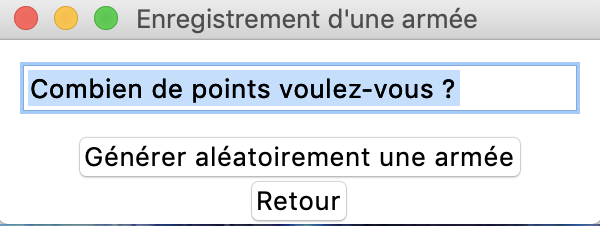
\includegraphics[width=5cm]{Images/pointsAleatoire.png} 
	\caption{Saisie du nombre de points pour création aléatoire d'armée\label{fig:pointsAleatoire}}
	\end{center}
\end{figure}

La génération d'une armée aléatoire fait appel à une méthode de classe qui génère une armée aléatoire en fonction d'un nombre de points donné : Figure \ref{fig:pointsAleatoire}. Les curseurs prennent la valeur correspondante au nombre d'unités de l'armée générée. Cette dernière est éditable par la suite par l'utilisateur. On accède aux valeurs des curseurs en parcourant le dictionnaire \texttt{scales} de l'objet SelectionTroupe puis à l'attribut $var$ déclaré dans la classe MonScale.\\

Les trois pages qui seront les plus fréquentées seront celles du menu solo, du menu multijoueur et du menu optimisateur.
\\
Dans les menus, le bouton Afficher armée permet d'afficher l'armée du joueur et ses caractéristiques. Si aucune armée n'a été sélectionnée, les statistiques valent simplement zéro. Il est possible de voir son nombre total de point d'attaque, de défense, de vitesse et le coût de l'armée. Les troupes sont également affichées avec le nombre et le type d'unité. Un texte est passé au constructeur de la classe LabelAffichage pour ajouter les labels des unités de façon identique. \\

Un paramètre est possible pour l'affichage des armées. En effet, lors de la récupération d'une armée, celle-ci est affichée avec cette méthode. Mais l'armée du joueur sélectionnée par l'utilisateur est déjà modifiée par l'armée récupérée. Si l'utilisateur s'est trompé d'armée, il peut revenir en arrière et cliquer sur "Quitter sans enregistrer" pour remettre l'armée d'origine stockée temporairement dans la fenêtre dans l'attribut \texttt{armeeTemp}.\\

Pour la récupération d'une armée dans un fichier, l'utilisateur doit donner le nom de l'armée ou la sélectionner via un explorateur. Un chemin vers le fichier est retourné et un test permet de vérifier s'il s'agit bien d'un fichier JSON. Si c'est le cas, l'effectif sérialisé dans le fichier est extrait et l'armée est créée. Elle peut servir à tous les utilisateurs comme on le voit dans la figure \ref{fig:RecuperationArmee}. L'armée est ensuite affichée à l'utilisateur avec l'option de quitter sans enregistrer.\\

Enfin, après avoir choisi son armée, l'avoir affichée ou encore l'avoir enregistrée, il est possible de la faire combattre. Pour cela, plusieurs types de combats sont possibles :
\begin{enumerate}
	\item Combat contre une armée aléatoire en solo
	\item Combat contre l'optimisateur après avoir généré une armée
	\item Un affrontement entre deux joueurs
\end{enumerate}

Pour le premier cas, il faut que le joueur solo possède une armée, puis sélectionne le combat contre aléatoire. Une armée aléatoire est générée, basée sur le nombre de points de celle de l'utilisateur et le combat démarre. Il utilise notre moteur de combat. Plusieurs images permettent de remarquer que le combat est en cours. Elles apparaissent avec un délai d'une seconde pour simuler une attente car le combat est rapide à calculer (voir \hyperref[performances]{la partie performances}. Le résultat est affiché à l'aide des frames de résultat chargées au lancement du programme.

Seconde option, il est possible de combattre contre l'IA en mode solo. Il ne faut pas oublier de créer une armée optimisée pour l'IA grâce à l'algorithme génétique que nous avons implémenté, puis lancer le combat. Des tests permettent d'indiquer à l'utilisateur quelle armée n'est pas formée, dans ce cas, le combat n'est pas lancé. Les deux armées s'affrontent et le vainqueur est déclaré. Les méthodes qui permettent de lancer ces affrontements sont dans la classe MaFen et lancées directement depuis les boutons des frames.

Pour l'optimisateur, le lancement s'effectue depuis son menu, la méthode \texttt{algo} de la classe MaFen va chercher les valeurs des boutons-radios dans les IntVar() et appeler la fonction de l'algorithme du module optimisateur. \label{InterfaceOptimisateur}
L'interface permet par ailleurs la visualisation que l'optimisation est en cours avec une barre de chargement. En effet, deux Threads sont lancés (méthode du multithreading). C'est à dire que l'ordinateur va exécuter deux codes en même temps : celui de l'algorithme génétique mais aussi celui de la barre de progression ajoutée à l'interface. Cette barre est créée avec un module de Tktiner : ttk puis ajoutée avec la méthode pack.
De plus, il est possible d'enregistrer directement l'armée générée dans un fichier JSON.
\\
La barre de progression marche de manière infinie, c'est à dire qu'elle va continuer à faire des allers-retours tant qu'elle n'est pas arrêtée ou détruite. Après avoir fini l'optimisation, elle est détruite. Elle fonctionne de la manière suivante : une barre est créée avec le widget ProgressBar : \texttt{ttk.Progressbar(frame, options)} puis on boucle avec la méthode start qui fait avancer le bandeau dans la barre : \texttt{progress.start(50)}. La barre est détruite à la fin de l'optimisation.\\

Enfin tous les boutons "quitter" sont mis en valeur avec un fond de couleur rouge issu d'une variable globale comprenant le code couleur. Il permet de fermer la fenêtre ou la Toplevel actuelle et donc de quitter le jeu proprement.\\

Dans le fichier main, le logo dans la barre des tâches de l'application est changé par la modification de l'iconphoto.

	\subsection{Structures de données}\label{structureDonnees}
Les structures de données permettent d'organiser les données du programme pour les traiter plus simplement et rapidement.\\

Le jeu est basé sur un système d'armées formées par l'utilisateur ou générée aléatoirement. Une armée est un objet Armee instancié depuis la classe Armee.
Une armée possède des attributs d'instance : des points de vie, d'attaque, de défense, de vitesse et un coût total sous forme d'entiers.
Elle possède également un dictionnaire de limites avec pour clé un nom de troupe et pour valeur le maximum de ce type d'unités.
Le dictionnaire 'troupes' comportera l'ensemble des troupes d'une armée après que cette dernière ait été formée. Il se présente sous la forme clé : nom de la troupe, valeur : liste d'objets Troupe qui correspondent à son nom.
Une armée est donc composée d'objets Troupe si elle n'est pas vide.\\

L'ajout des troupes dans l'armée est fait depuis une méthode de l'objet Armee en lui passant un effectif sous forme de dictionnaire (clé : nom, valeur: nombre unités souhaité). Une boucle se charge d'instancier les troupes une à une avec le constructeur de la classe Troupe puis placée dans la liste correspondante à son nom dans l'armée. On a donc une armée constituée d'un dictionnaire troupes qui comporte des listes d'objets Troupes qui possèdent chacune ses propres caractéristiques.\\

Les valeurs spécifiques à une troupe se trouvent dans l'attribut de classe carac de la classe Troupe. Tout ajout ou suppression de troupes pour le programme se fait dans ce dictionnaire.\\

Une armée contient une hiérarchie pour détruire les unités dans un ordre précis. Elle est sous la forme d'une liste ordonnée où le premier nom contenu sera l'unité qui succombera en premier lors d'un affrontement.\\

L'interface graphique utilise des variables propres au module Tkinter. Elles sont déclarées par l'appel d'un constructeur de classe du type IntVar() ou StringVar(). Ces variables sont directement liées au widgets et permettent d'actualiser leur valeur de manière graphique lorsqu'elle changent.\\

L'interface graphique permet par ailleurs de sérialiser les armées dans des fichiers JSON pour être réutilisées par la suite. Ces fichiers contiennent un dictionnaire avec pour clé le nom de la troupe et pour valeur un entier correspondant au nombre de troupes. Ce fichier n'est pas une armée mais un effectif qu'il est possible d'ajouter à une armée par la suite via les méthodes associées.

	\subsection{Bibliothèques}\label{bibliothèques}
Les bibliothèques nous permettent d'utiliser des méthodes qui faciliteront la programmation du programme. Voici les bibliothèques que nous avons utilisées pour réaliser notre projet : 
\begin{itemize}
	\item Pour le moteur de combat : random, time 
	\item Pour l'algorithme génétique : copy, time 
	\item Pour la partie graphique : tkinter, Pil, json, os.path, copy, time, threading, tkinter.filedialog, tkinter.messagebox
\end{itemize}

\newpage
\section{Architecture du projet}
	\subsection{Architecture globale des dossiers et des fichiers}
Voici l'architecture de notre projet :

\makeatletter
\newcount\dirtree@lvl
\newcount\dirtree@plvl
\newcount\dirtree@clvl
\def\dirtree@growth{%
  \ifnum\tikznumberofcurrentchild=1\relax
  \global\advance\dirtree@plvl by 1
  \expandafter\xdef\csname dirtree@p@\the\dirtree@plvl\endcsname{\the\dirtree@lvl}
  \fi
  \global\advance\dirtree@lvl by 1\relax
  \dirtree@clvl=\dirtree@lvl
  \advance\dirtree@clvl by -\csname dirtree@p@\the\dirtree@plvl\endcsname
  \pgf@xa=0,5cm\relax
  \pgf@ya=-0,45cm\relax
  \pgf@ya=\dirtree@clvl\pgf@ya
  \pgftransformshift{\pgfqpoint{\the\pgf@xa}{\the\pgf@ya}}%
  \ifnum\tikznumberofcurrentchild=\tikznumberofchildren
  \global\advance\dirtree@plvl by -1
  \fi
}

\tikzset{
  dirtree/.style={
    growth function=\dirtree@growth,
    every node/.style={anchor=north},
    every child node/.style={anchor=west},
    edge from parent path={(\tikzparentnode\tikzparentanchor) |- (\tikzchildnode\tikzchildanchor)}
  }
}

\begin{figure}[h]
\begin{center}
\begin{tikzpicture}[dirtree]
\node {src} 
    child { node {Armee.py} }
    child { node {interface.py} }
    child { node {Troupe.py} }
    child { node {moteurCombat.py} }
    child { node {optimisateur.py} }
    child { node {FAQ.txt} }
    child { node {Regles.txt} }
    child { node {main.py} }
    child { node {Images}
    		child { node {combat\_en\_cours1.gif} }
    		child { node {combat\_en\_cours2.gif} }
    		child { node {victoire.gif} }
    		child { node {defaite.gif} }
    		child { node {egalite.gif} }
    		child { node {victoire\_joueur1.gif} }
    		child { node {victoire\_joueur2.gif} }
    		child { node {icon.png} }
   	    };
\end{tikzpicture}
\end{center}
\caption{Arborescence des dossiers}
\end{figure}

	\subsection{Architecture des modules et des classes}
Figure en annexe \ref{Annexe A} Figure \ref{fig:DiagClasses}.
La Classe MaFen est la classe principale, elle utilise l'ensemble des classes qui héritent de Frames, Toplevel, Scale et Label pour l'affichage. La classe MaFen hérite de l'objet Tk, la fenêtre graphique de Tkinter. 
De plus, elle utilise la classe Armee et notamment la méthode de génération aléatoire d'effectif. Une armée peut être composée d'une ou plusieurs troupes qui proviennent de la classe Troupe. Les méthodes sont indiquées et les attributs de classe également. Cependant, les attributs d'instance ne sont pas représentés sous peine de surcharger la figure.
Les modules utilisés ne sont pas représentés, mais les modules \texttt{moteurCombat} et \texttt{optimisateur} sont nécessaires pour faire combattre les armées et lancer une optimisation. La classe MaFen utilise donc ces modules pour permettre d'utiliser toutes les fonctionnalités. Des bibliothèques sont nécessaires et importées directement dans les fichiers, elles sont détaillées dans la partie \ref{bibliothèques}.

\section{Expérimentations, usages et performances}
	\subsection{Expérimentation et usages}
Au fil de notre projet, nous avons dû faire quelques expérimentations pour essayer d'implémenter de nouvelles fonctionnalités. En voici quelques-unes : 
\begin{itemize}
\item Expérimentations sur la partie moteur de combat : nous avions commencé à coder un moteur de combat qui pourrait supporter trois armées ou plus mais nous avons rapidement vu qu'il fallait totalement changer les règles d'engagements (chaque armée attaque l'armée à sa droite ou à sa gauche ou bien un nombre aléatoire permet de savoir qui attaque en premier). De plus, l'ajout d'un plateau de jeu serait alors nécessaire.
\item Expérimentations sur la partie graphique : nous avons tenté de mettre des images de fond sur lesquelles apparaissent des boutons mais nous n'avons pas réussi. La méthode classique est d'utiliser la méthode \texttt{pack} pour l'image et les boutons sur un canvas mais cela n'a pas fonctionné.
\item L'utilisation du programme varie en fonction du nombre de personnes.
\end{itemize}

	\subsection{Mesures de performance}\label{performances}
	Les performances de l'optimisateur sont primordiales car l'utilisateur ne peut pas patienter plusieurs dizaines de minutes pour générer une armée performante. Cependant il est possible d'augmenter ce temps de manière considérable en fonction des paramètres choisis pour le lancer. Certains paramètres sont plus influents que d'autres.
	
Pour mesurer ces temps d'exécution nous avons utilisé le module time et la fonction \%timeit.
\begin{enumerate}
\item Comparaison du temps d'exécution entre une IA faible et une IA forte : 
	\begin{itemize}
	\item La différence de temps d'exécution entre les deux compétences de l'IA passe du simple ou double de temps pour une IA Forte. Plus le nombre de points de l'armée sera grand, plus le temps d'exécution sera long.
	\end{itemize}

\item Comparaison du temps d'exécution des différents niveaux de l'IA : 
	\begin{itemize}
	\item Les niveaux 1 et 2 donnent des résultats au niveau temps presque identiques. Ce sont les niveaux les plus rapides. Cependant si l'utilisateur souhaite pousser l'optimisation, le niveau 3 est plus performant mais multiplie par 5 le temps d'optimisation par rapport aux deux premiers niveaux. Enfin, le niveau 4 triple ce temps d'exécution du niveau 3 car le nombre de combats que le programme doit réaliser est conséquent.
	\end{itemize}

\item Comparaison du temps d'exécution avec ou sans croisements multi-points : 
	\begin{itemize}
	\item Les croisements multi-points doublent le temps d'exécution. Ces croisements génèrent un combat supplémentaire à chaque tour puis les croisements entre les armées performantes s'effectuent.
	\end{itemize}

\item Comparaison du temps d'exécution avec l'algorithme d'évaluation : 
	\begin{itemize}
	\item L'algorithme d'évaluation se base sur un nombre de combats victorieux de l'armée minimum. C'est un test final qui donne ce résultat sans prolongement de temps d'exécution.
	\end{itemize}
\end{enumerate}

De plus, les combats entre armées doivent être rapides pour accélérer l'optimisation. La durée d'un combat est située en moyenne autour de $4.6ms$ pour deux armées de 2500 points et de $15.5ms$ pour des armées de 10000 points.

Pour finir, l'optimisateur à besoin de générer des armées aléatoires, elles sont rapides à créer mais cela varie en fonction du nombre de troupes. Ainsi, pour l'instanciation, création de l'effectif et ajout des troupes dans l'armée, on arrive à une moyenne de $0.9ms$ pour une armée de 2500 points et $3.2ms$ pour des armées de 10000 points.

En cumulant la création de deux armées puis leur combat, on arrive à une moyenne de $6.1ms$ de temps d'exécution pour deux armées de 2500 points et on monte à $22.7ms$ pour des armées de 10000 points.

\section{Conclusion}
	\subsection{Propositions d'amélioration}
Pour conclure, nous vous proposons plusieurs fonctionnalités qui pourraient participer à l'amélioration de notre projet :
\begin{itemize}
        \item Moteur de combat supérieur à deux armées : cela permettrait de faire des combats à plus de deux joueurs, voire de totalement modifier la manière dont les combats s'opèrent.
        \item Une interface graphique avec des animations : pour cela il faudrait changer de bibliothèque graphique.
        \item Rajouter une musique de fond : aucune musique de fond n'a été implémentée car les machines de la faculté ne permettent pas d'avoir du son.
        \item La possibilité de rajouter une unité depuis l'interface : après de multiples essais, nous avons réussi à ajouter une unité uniquement en ligne de commande.
        \item La possibilité de supprimer une unité de base : actuellement nous n'avons pas tenté de le réaliser.
        \item Le survol de la souris sur une unité depuis la création d'armées permet de voir ses caractéristiques : cela nous demanderait de ne plus utiliser Tkinter.
        \item L'ajout d'images pour visualiser les différents troupes possibles : Il faudrait pour cela créé les images unes à unes et de les ajouter au programme.
        \item Une visualisation concrète du combat : Nous pourrions le faire si nous avions des images et que nous les animions. 
        \item Lors de la sélection d'une armée, les curseurs prennent la position de l'armée courante pour la modifier légèrement et un bouton mise à zéro permet de la réinitialiser.
        \item Amélioration de l'algorithme génétique : l'ajout de nouvelles fonctionnalités serait un plus au programme mais pas au temps d'exécution. L'utilisation de bibliothèques spécifiques comme TensorFlow ou Scikit-Learn pourrait améliorer la performance de l'algorithme.\\
\end{itemize}

La possibilité de créer un optimisateur de wargame a été pour nous un excellent moyen de découvrir la programmation orientée objet en python. Elle nous a aussi prouvé que nous pouvions nous en sortir seul en programmation sur de simples projets. Il faut pour cela de la pugnacité, de l'envie, du travail et de l'audace.
\newpage
\begin{appendix}
    \section{Annexe}
    \subsection{Diagramme de classes}
    \label{Annexe A}
    \begin{figure}[!h]
	\begin{center}
	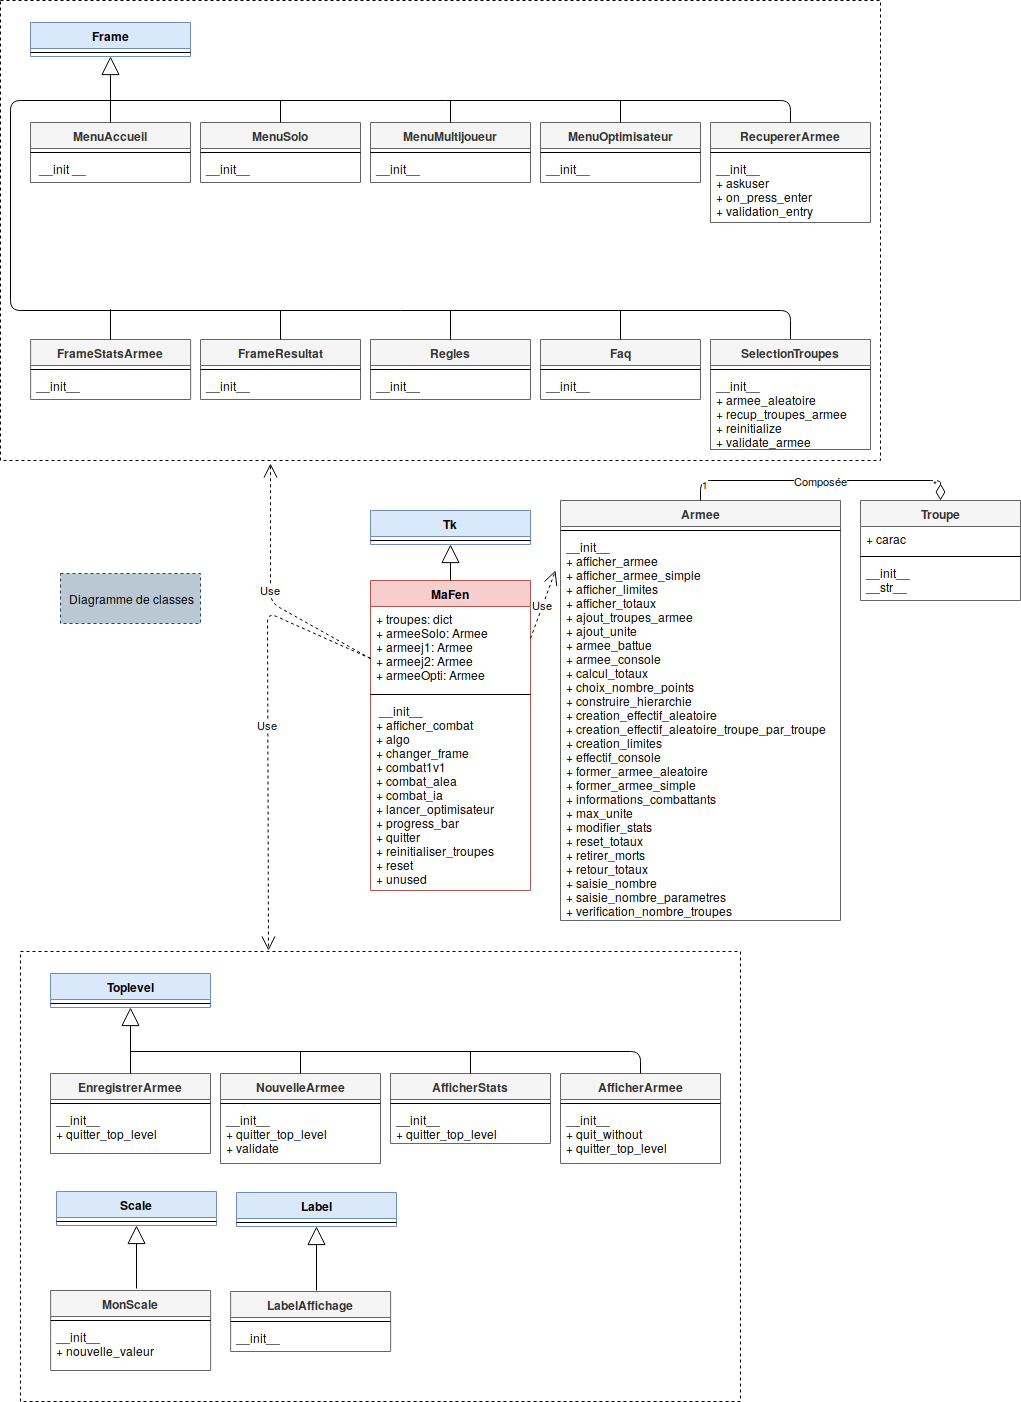
\includegraphics[width=16cm]{Images/diagramme-de-classes.png}
	\caption{Diagramme de classes\label{fig:DiagClasses}}
	\end{center}
	\end{figure}
\end{appendix}

\end{document} %fin du document

